% Shared manuscript body for the closed-loop substrate validation.
% Included by main.tex (signed) and main_anon.tex (double-anonymous).
%
% ICRA 2027 style: 8 pages including references, double column.

\usepackage{cite}
\usepackage{amsmath,amsfonts,amssymb}
\usepackage{graphicx}
\usepackage{textcomp}
\usepackage{booktabs}
\usepackage{array}
\usepackage{multirow}
\usepackage{url}

\title{Closed-Loop Task Function Across a Spiking Culture Substrate on a
Humanoid: A Load-Bearing Demonstration with Ablations, Information-theoretic
Evidence, and Physical Boundaries}

\AuthorsBlock

\begin{document}

\markboth{Closed-Loop Task Function Across a Spiking Culture Substrate}{}
\maketitle

\begin{abstract}
Can a control function that must perform a physical task actually travel
through a spiking culture substrate and back into a robot, such that the loop
is load-bearing rather than cosmetic? We instrument a Unitree G1 humanoid in
MuJoCo with the full measurement contract of a closed-loop cortical platform
(sixty-four electrode channels at 25\,kHz, a spike threshold, committed
stimulation) and close the loop through two biological-style substrates: a
rate-code transducer and an Izhikevich microcircuit. Sensor state is encoded
to electrodes; spikes are read from the substrate; a fixed Nengo-LIF hub
decodes a forward-velocity command that is stimulated back onto the plant.
Against five velocity task profiles, five experimental modes, and six seeds,
the intact loop tracks the commanded profile significantly better than a zero
command, an uncoupled random decoder, a 50\,\% electrode lesion, and a dead
Poisson substrate whose spikes are statistically matched but carry no state
information (exact paired permutation $p \leq 0.0156$ on every profile and
every null). The ordering replicates across substrate change and is
corroborated by mutual information and transfer entropy along the causal chain
electrode$\rightarrow$spikes$\rightarrow$command, and by signed,
terrain-dependent changes in real walking outcomes. A causal walk-forward
readout of the recorded spike streams finds task information in the intact
substrate significant against the statistically matched dead substrate
(one-sided paired $p=0.015$ for the rate-code substrate, $p<0.001$ for the
Izhikevich substrate) while no substrate supports a linear readout above a
trivial predictor---the behavioral separation is a whole-loop property whose
boundaries we measure rather than assume. We also report the loop's physical
authority boundary and its information latency honestly. All software, assets,
raw trials, and analysis code are released as a single public repository.
\end{abstract}

\begin{IEEEkeywords}
substrate computing, spiking neural networks, closed-loop control, humanoid
locomotion, mutual information, transfer entropy, falsification.
\end{IEEEkeywords}

\section{Introduction}

A recurring empirical claim in the wetware-embodiment literature is that a
dish of cultured cortical neurons, interfaced with a simulated environment,
can \emph{learn} a game-like task
\cite{kagan2022dishbrain}. The claim is important if true, because it would
mean a non-gradient, substrate-native computation could perform a task function
in a closed loop. It is also contested on conceptual and statistical grounds
\cite{balci2023neurons,kagan2023semantics}. Two weaknesses repeat across the
discussion. First, claims are usually about the substrate \emph{learning}
something, while the supporting evidence is an open-loop firing-rate change, an
admitted novelty mechanism, or a single unablated game score; a falsifiable,
load-bearing arrangement is rarely shown. Second, the loop itself is usually
not scrutinized: when a ``brain'' reports a command and a game or robot
appears to move, the information that actually drove the movement may live in
the readout and in the environment, not in the spikes
\cite{embodied_neurocomp}. A task function that demonstrably requires the
substrate, and whose destruction under ablation is measurable, is the missing
demonstration in either direction.

This paper constructs that demonstration for a load-bearing control task, in
simulation, using the measurement contract of a closed-loop culture platform.
A Unitree G1 humanoid walker in MuJoCo is driven by a trained policy, and a
velocity-tracking task is closed through a spiking substrate: sensory state is
encoded to electrode frames, a substrate emits spike events, and a small fixed
spiking hub decodes them into a stimulation that modulates the walker's
forward velocity. The task channel is a designated electrode, so the commanded
velocity profile must physically traverse the substrate--spike--decode--stim--
plant chain. We attached to this loop the strongest falsification apparatus we
could build without leaving simulation:

\begin{itemize}
\item a five-profile, five-mode, six-seed battery with exact paired permutation
      statistics, whose $p$-value floor ($1/64$) is dictated by the seed count
      and reported as such;
\item a dead-substrate null (Poisson draws matched in spike rate but carrying
      no state), an uncoupled-decoder null, a zero-command null, and a
      50\,\% electrode lesion;
\item information-theoretic evidence (mutual information and transfer entropy)
      along the causal chain, bias-corrected against a shuffle null;
\item substrate interchangeability: the same closed loop on a second, genuinely
      dynamical spike source (an Izhikevich microcircuit), at full power;
\item physical boundaries: terrain-induced, statistically signed changes in
      survival and traveled distance, a measured authority frontier under
      lateral impulses, and an explicit information-latency figure on the
      critical path.
\end{itemize}

The contribution is therefore not an effect size but a falsifiable protocol:
the loop is load-bearing if and only if ablation can destroy its function in
the ways listed, and it fails honestly at the boundaries we report. We are
also explicit about what is \emph{not} shown even after the full battery: the
closed-loop readout-invariance gate (Section~\ref{sec:resG}) measures that the
best causal linear readout of the recorded spikes never beats a trivial
window-mean predictor for any mode, and that the spike$\rightarrow$command edge
does not survive as linear structure---yet the intact substrate carries task
information above a statistically matched dead substrate at paired significance
in both substrates. The load-bearing claim therefore survives; the stronger,
readout-invariant reading is rejected by measurement, not assumed.

\section{Related Work}

\emph{Cultured platforms.} DishBrain demonstrated that dissociated cortical
neurons can be driven by a simulated Pong environment through a high-density
multielectrode interface \cite{kagan2022dishbrain}; the subsequent
methodological reply \cite{balci2023neurons} and semantics exchange
\cite{kagan2023semantics} framed the standards of evidence. Brain organoid
reservoir computing showed that organoid activity can serve as a dynamical
readout for a benchmark task \cite{cai2023brainoware}. The present work shares
the ``embodied task through electrodes'' structure but differs in emphasis: we
hold the substrate's \emph{contribution} constant and destroy it deliberately,
quantifying what breaks.

\emph{Spiking substrates.} Spiking networks are the accepted third-generation
computational model \cite{maass1997}; the Izhikevich neuron efficiently spans
the known single-neuron repertoire \cite{izhikevich2003,izhikevich2004}. Liquid
state machines showed that a fixed, untrained recurrent reservoir supports
real-time computation when a trained readout exists \cite{maass2002liquid},
which is precisely the configuration we use and the reason decoder-invariance
\cite{embodied_neurocomp} is a first-order threat to such claims. The Neural
Engineering Framework and its Nengo implementation provide the principled
Kernel of our readout: represent a function of the spike population via a
linearly optimal decoder \cite{eliasmith2003,bekolay2014}.

\emph{Closed-loop validation.} Our falsification battery follows the protocol
of our companion work \cite{embodied_neurocomp}, which introduced a
falsification-style gate structure for embodied spiking substrates and
demonstrated open-loop that apparent tracking can survive only under a held-out
readout. The physiological literature on population decoding
\cite{georgopoulos1986,quiroga2009,paninski2004} and on information measures in
spike trains \cite{schreiber2000,kraskov2004,panzeri2007,walker2018} provides
the analytical tools; exact permutation inference \cite{ernst2004},
surrogate-data testing \cite{theiler1992}, and the pseudoreplication caution
\cite{hurlbert1984} anchor the statistics. Physically, MuJoCo
\cite{todorov2012} and the Unitree RL-Gym policy deployment stack
\cite{unitree_rl_gym} supply the plant; our contribution is the substrate
contract and the experimental design layered on top.

\section{System}

\subsection{The substrate contract}

The loop uses the data-source contract of a closed-loop cortical platform:
sixty-four electrode channels, frames at 25\,kHz, a per-sample amplitude unit of
0.195, and stimulation committed per channel. Every tick of the outer loop
(40 ticks/s, i.e. a 25\,ms contract tick) exposes the last block of electrode
frames to the substrate and collects its spike events; a stimulation on a
designated channel is applied back to the plant within the same tick. Spikes
are counted as downward threshold crossings of $-1400$ (sample units) across
consecutive frames, a deliberately simple and inspectable event definition.

Channel roles: electrodes 0--11 carry normalized joint tracking error (torque
overlay, amplified $40\,\mathrm{N\,m}$ per decoder unit); 12--13 carry roll and
pitch; 23 carries pelvis height; 62 is the \emph{task channel}---commanded
forward velocity injected as the load-bearing input; 63 is a hub-context
electrode. All other channels remain at noise.

\subsection{The plant}

The plant is the Deploy12 G1 loader: a 12-DoF Unitree G1 humanoid, a frozen
LRRT policy checkpoint, an analytic PD tracker, and a MuJoCo simulation at
2\,ms with control decimation 10 (50\,Hz). The datasource advances physics
across control boundaries inside its \texttt{read()} call and applies
committed stimulations in \texttt{on\_stim()}; channel 62 stimulation maps to a
forward-velocity override on the policy's command input
($4\,\mathrm{uA}$ per $\mathrm{m/s}$), capped at $0.75\,\mathrm{m/s}$, so the
task channel truly moves the body. Reference conditions run the identical
plant with no neural command.

\subsection{Substrates}

\textit{Rate-code transducer.} Each of the 64 channels encodes its sensor value
into a renewing sinusoidal transient whose amplitude grows and whose interval
shrinks with $|s|$, superimposed on per-channel noise. This is a minimal
``fiery-when-offset'' rate code whose only job is to read the electrode
contract.

\textit{Izhikevich microcircuit.} A per-channel group (six regular-spiking,
two fast-spiking Izhikevich neurons) integrates the sensor drive; volleys are
counted into the same 25\,kHz frames. The drive gain is calibrated so the
per-channel volley counts match the rate-code substrate across the sensor
range (ratio 0.78--1.04), isolating \emph{substrate dynamics}---not spike
rate---as the manipulated variable. Both substrates run in-process, stateless
across ticks, seeded per run.

\subsection{Decision hub}

The readout is a Nengo network: a 1000-neuron LIF (Leaky-Integrate-and-Fire)
ensemble encoding the five-dimensional state
$[\,\mathrm{roll},\ \mathrm{pitch},\ \mathrm{thsig},\ n_{\mathrm{spk}},\ \mathrm{ctx}\,]$,
decoded to the two-dimensional command $[v_x,\ \tau]$ through the fixed
function $\mathrm{decide}$:

\begin{equation}
\begin{aligned}
\mathrm{gate} &= \sigma\bigl(30\,(n_{\mathrm{spk}} - 0.15)\bigr), \\
\mathrm{slow} &= 1 - 0.9\,\sigma\!\bigl(10\,(\lvert\mathrm{roll}\rvert \vee
\lvert\mathrm{pitch}\rvert - 0.9)\bigr), \\
v_x &= \mathrm{clamp}\!\Bigl(\tfrac{\mathrm{thsig} - 0.0615}{0.277},
0.0,\ 0.75\Bigr) \cdot \mathrm{gate}\cdot \mathrm{slow}, \\
\tau &= 0.75 \cdot \tanh\bigl(2\,\mathrm{roll}\bigr).
\end{aligned}
\end{equation}

The hub runs at 2\,ms in chunks of 600 steps (1.2\,s of hub time per chunk) to
amortize per-call overhead; the decoded command is read from the most recent
chunk. The gap between the spike window that produced a command and its
application is the loop's information latency (Section~\ref{sec:resE}).

The hub is \emph{not} trained on the task; it is a fixed, manually specified
decode of spike counts. This is deliberate: the substrate must prove itself as
the carrier, so we keep the readout constant across all modes and both
substrates.

\section{Protocol}

\subsection{Task-tracking battery}

Every run lasts 12\,s (500 outer ticks) on flat ground. The task is a velocity
profile injected on channel 62; five profiles are used: \emph{baseline}
(0.5$\rightarrow$0.8$\rightarrow$0.5\,m/s), \emph{multi\_step}, \emph{sine},
\emph{descend}, and \emph{pulse}. Five modes are compared per profile:
\texttt{neural} (intact loop), \texttt{zero} (no command issued), \texttt{random}
(uncoupled fixed random decoder), \texttt{mask0.5} (50\,\% of electrodes zeroed
per seed, i.e.\ a lesion that can erase the task channel itself), and
\texttt{poisson} (frames replaced by a Poisson process with the same expected
spike rate but no dependence on state). Six seeds
$\{1,7,13,29,55,91\}$ fix the simulator RNG, the noise/event RNG, and the
lesion draw; the hub is deterministic, so seed variance reflects the substrate,
the plant, and real-time timing.

Primary outcome: tracking RMSE between the applied command and the profile. With
six seeds the best possible one-sided exact permutation $p$ is $1/64$ and the
two-sided is $2/64$ \cite{ernst2004}; we report both p and the paired effect
size $d_z$.

\subsection{Information-theoretic gate (Gate~A)}

Additionally capturing per-tick spike counts and plant state for all five modes
(two seeds), we estimate mutual information $\mathrm{MI}(\mathrm{cmd};\mathrm{plant})$
with the Kraskov--St\"ogbauer--Grassberger estimator \cite{kraskov2004} and
transfer entropy \cite{schreiber2000} along the causal chain
$c_{62}\rightarrow\mathrm{cmd}$ and
$\mathrm{spikes}\rightarrow\mathrm{cmd}$, at lags 1--8. Both are
bias-corrected against a shuffle null
\cite{panzeri2007,walker2018} and reported in nats.

\subsection{Substrate interchangeability (Gate~B)}

The full battery is repeated with the Izhikevich substrate in place of the
rate-code transducer, same profiles, modes, seeds, and statistics. This tests
whether the closed-loop ordering is an artifact of the particular pattern
generator.

\subsection{Terrain and authority envelope}

Three non-flat MuJoCo scenes ($2^{\circ}$ ramp, 5\,cm curb, rough bumps) run the loop
under a constant $0.5\,\mathrm{m/s}$ march duty, comparing the neural closed
loop against the reference policy. Statistics: Fisher exact test for survival,
Welch $t$-test for traveled distance. A lateral impulse frontier and a
sustained-push torque probe establish the loop's physical authority envelope,
and the per-tick cadence is recorded to verify the 25\,ms contract deadline.
Each run also records whether the walker falls.

\section{Results}

\subsection{Task tracking}
\label{sec:resA}

Table~\ref{tab:tracking} shows the primary battery (rate-code substrate) and
Fig.~\ref{fig:tracking} juxtaposes it with the Izhikevich replicate. On all five
profiles and against all three nulls, the intact loop is significantly better:
6/6 seeds point the same way, giving $p=0.0156$ one-sided
($p=0.03125$ two-sided) on every comparison---the $p$-value floor for six
seeds---with large paired effect sizes (baseline $d_z=-38.9$ vs.\ zero,
$-8.6$ vs.\ random, $-2.4$ vs.\ mask0.5; range across profiles
$d_z\in[-2.4,-3.0]$ vs.\ mask0.5).

Note the ordering the ablations enforce. \texttt{zero} scores the profile itself
($\approx 0.6$): it is a floor, not a control. \texttt{random} improves on zero
because \emph{an uncoupled decoder that merely emits pressure toward the
profile direction} already drives the base policy's stability; this is exactly
why random must be present---a naive ``brain \emph{vs}.\ no brain'' comparison
cannot separate the decoder's coupling from the substrate's information. The
dead substrate \texttt{poisson} sits strictly between \texttt{neural} and the
uncoupled modes on every profile: statistically matched spikes, but no state,
track worse than the intact spikes. The 50\,\% lesion degrades the decode by
$+40$--$+96\,\%$ RMSE and in some seeds erases channel 62 entirely, which is the
mechanism by which the task signal disappears.

\begin{table}[t]
\centering
\caption{Tracking RMSE (mean$\pm$std) by profile and mode, rate-code substrate,
six seeds. Braces bold the best mode per profile.}
\label{tab:tracking}
\small
\begin{tabular}{lccccc}
\toprule
Profile & \texttt{neural} & \texttt{zero} & \texttt{random}
        & \texttt{mask0.5} & \texttt{poisson}\\
\midrule
baseline & \textbf{0.238$\pm$0.010} & 0.612$\pm$0.000 & 0.337$\pm$0.004
         & 0.397$\pm$0.057 & 0.306$\pm$0.006\\
multi\_step & \textbf{0.234$\pm$0.006} & 0.606$\pm$0.000 & 0.329$\pm$0.005
         & 0.383$\pm$0.057 & 0.297$\pm$0.003\\
sine & \textbf{0.241$\pm$0.005} & 0.601$\pm$0.000 & 0.333$\pm$0.007
         & 0.387$\pm$0.052 & 0.307$\pm$0.005\\
descend & \textbf{0.258$\pm$0.009} & 0.644$\pm$0.000 & 0.358$\pm$0.005
         & 0.424$\pm$0.058 & 0.336$\pm$0.003\\
pulse & \textbf{0.216$\pm$0.012} & 0.554$\pm$0.000 & 0.294$\pm$0.008
         & 0.344$\pm$0.045 & 0.252$\pm$0.006\\
\bottomrule
\end{tabular}
\vspace{2pt}
\begin{flushleft}
\footnotesize
Per comparison (5 profiles $\times$ 3 nulls, paired over seeds):
$p_{\mathrm{1s}}=0.0156$, $p_{\mathrm{2s}}=0.03125$ (all 6/6 same direction).
\end{flushleft}
\end{table}

\begin{figure}[t]
\centering
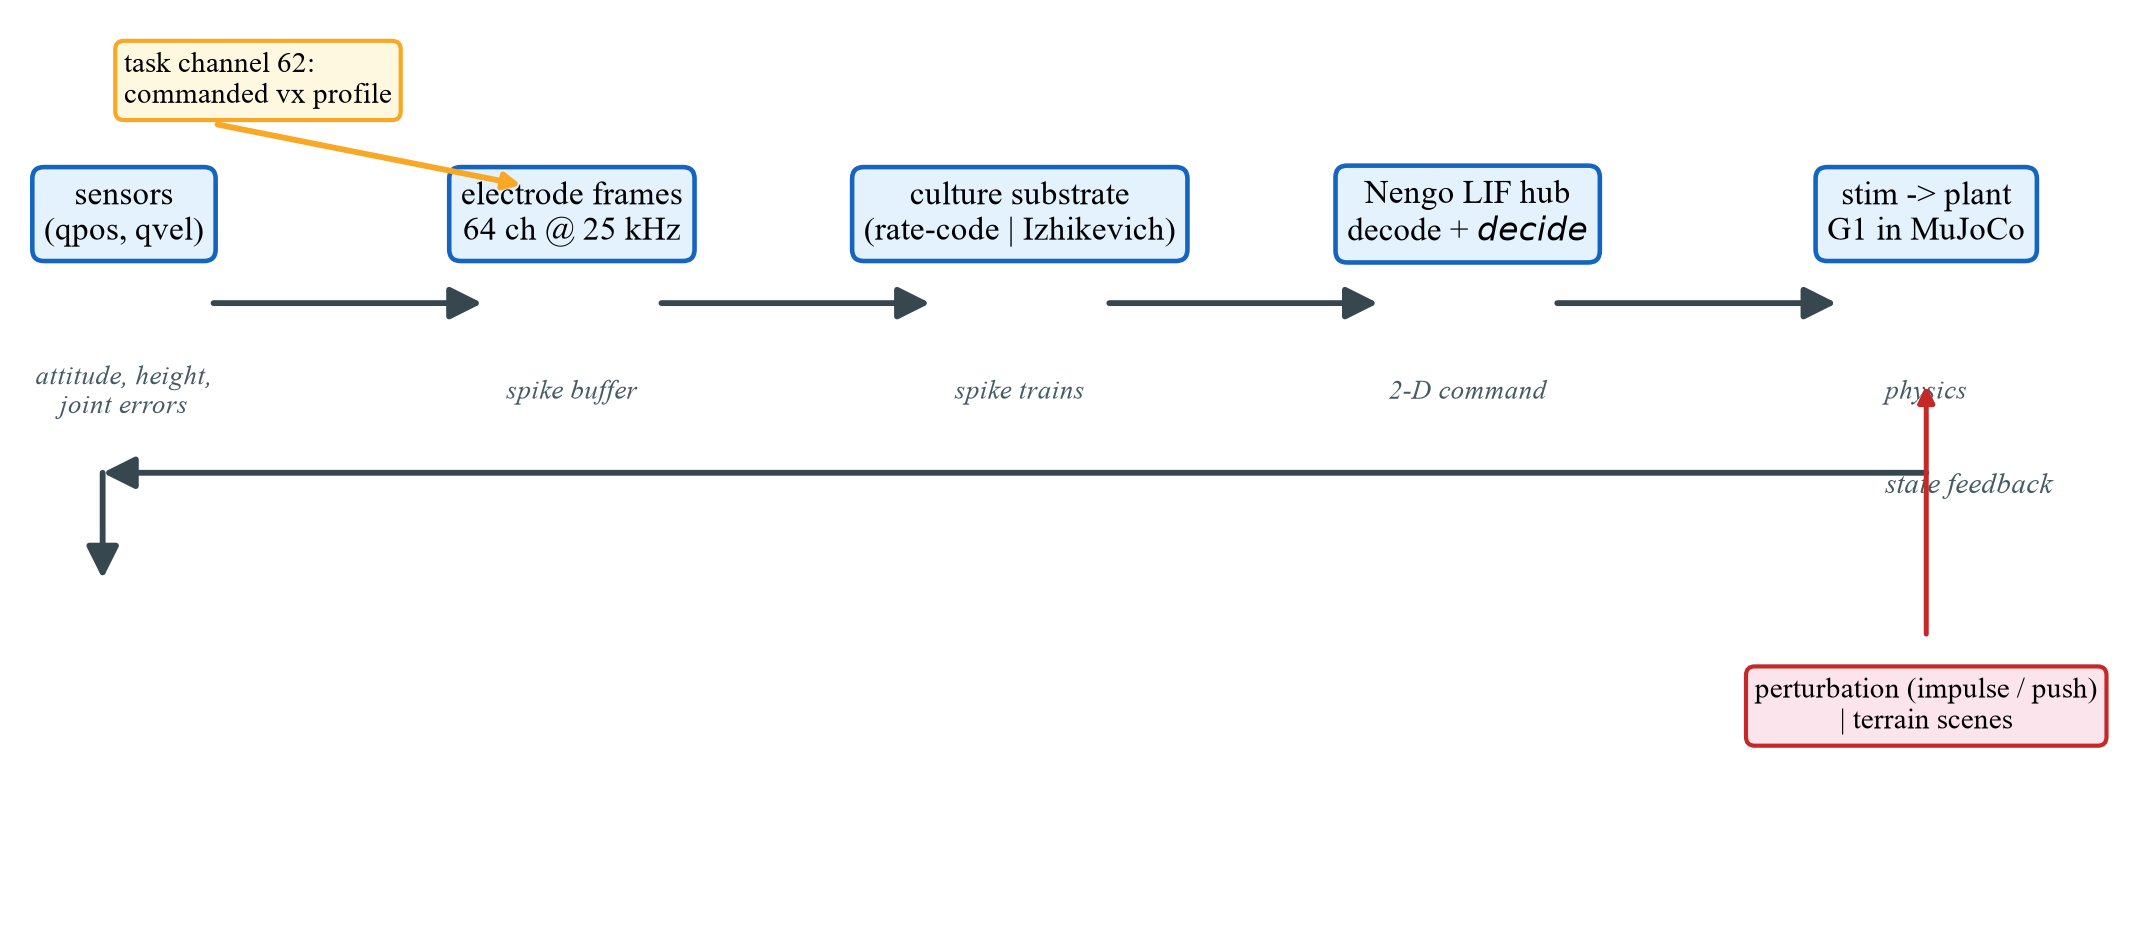
\includegraphics[width=\columnwidth]{figures/fig1_pipeline.png}
\caption{The closed loop. Task channel 62 injects the velocity profile; sensor
state is encoded to electrode frames; the substrate (rate-code or Izhikevich)
emits spikes; the fixed LIF hub decodes a command; stimulation commits it back
onto the plant in contract time. Null modes cut exactly one link in this
chain.}
\label{fig:pipeline}
\end{figure}

\begin{figure*}[t]
\centering
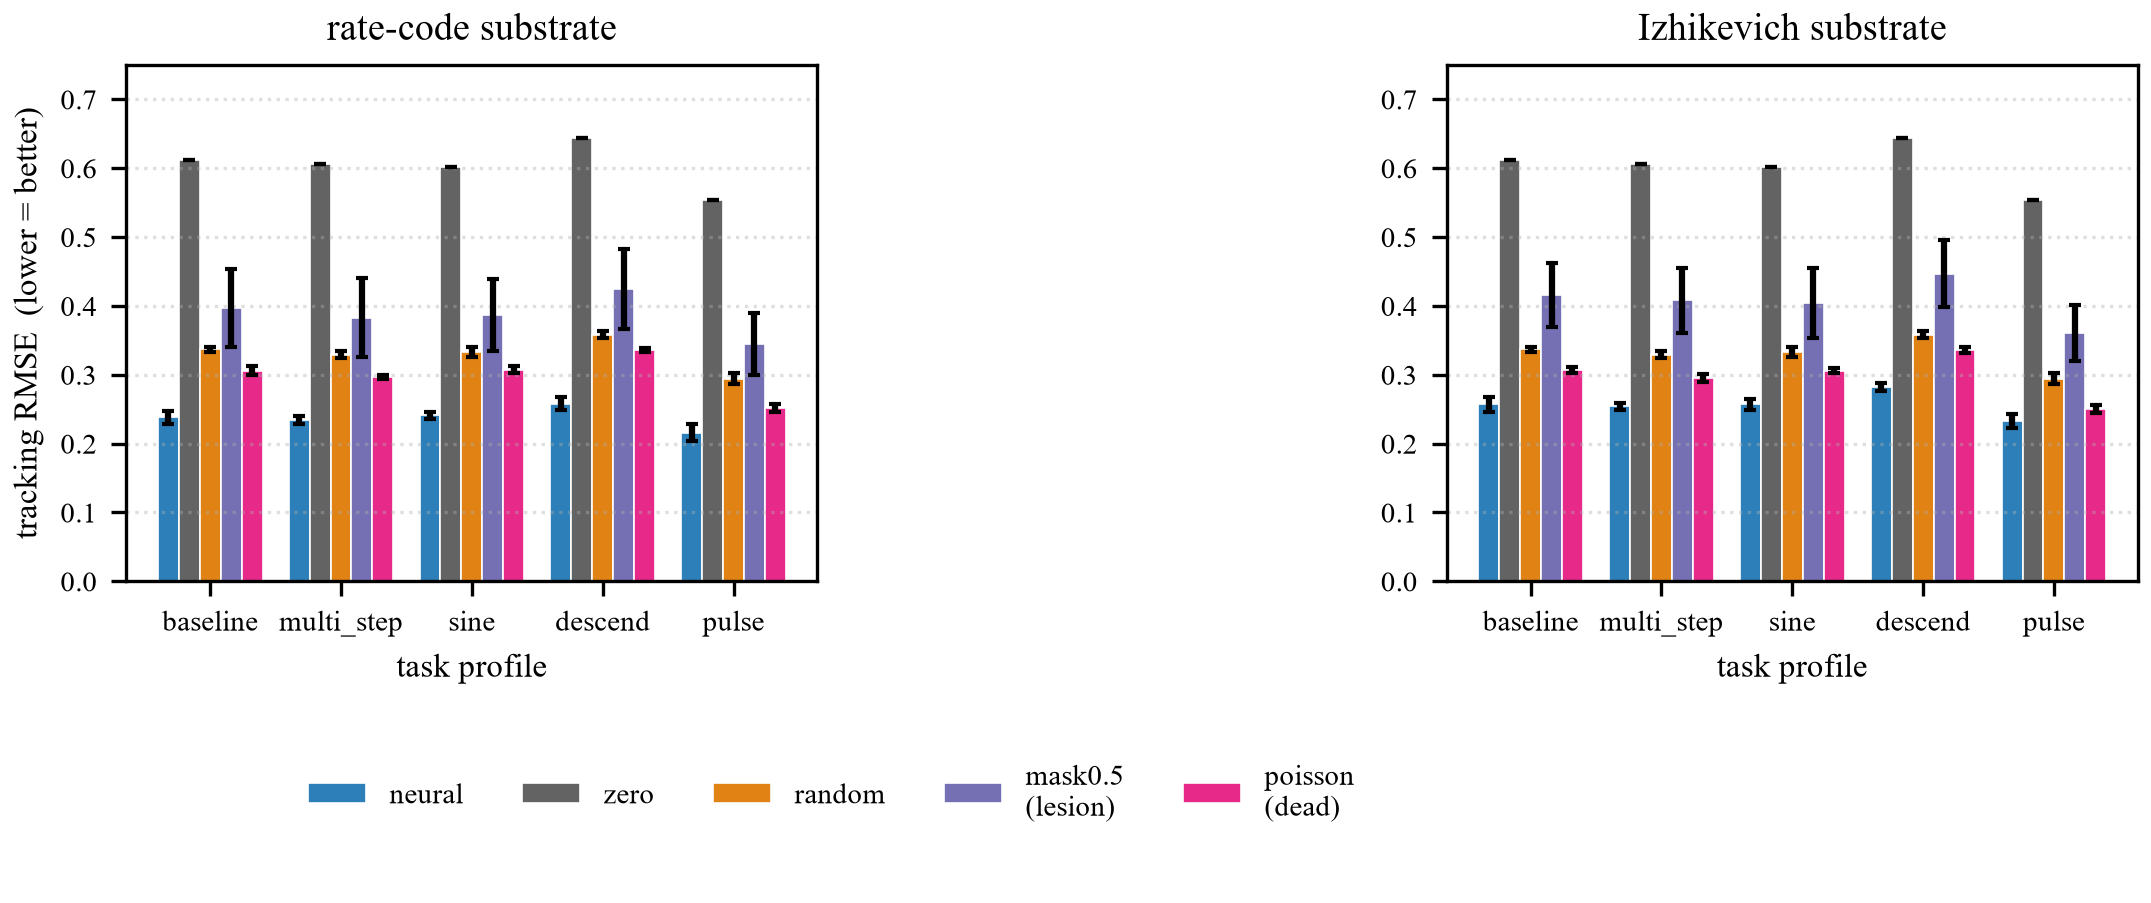
\includegraphics[width=\textwidth]{figures/fig2_tracking.png}
\caption{Tracking RMSE by profile and mode for the rate-code (left) and
Izhikevich (right) substrates, six seeds, error bars$\pm$1\,sd. On every profile
the intact loop is best and the dead substrate lies strictly between the intact
and the uncoupled/lesioned modes.}
\label{fig:tracking}
\end{figure*}

\subsection{Information-theoretic evidence (Gate~A)}
\label{sec:resB}

Table~\ref{tab:gate} reports MI and TE. Three readings matter.

First, $\mathrm{MI}(\mathrm{cmd};\mathrm{plant})$ is maximal for the intact
loop and zero for the uncoupled decoders: the task signal exists in the plant
only when the decoder is coupled to the substrate. Second, transfer entropy
along $c_{62}\rightarrow\mathrm{cmd}$ is nonzero only for the intact loop and
exactly zero for \texttt{zero}, \texttt{mask0.5}, and the dead substrate---the
causal chain through the spikes is present for the substrate that carries state
and absent otherwise. Third, both quantities reproduce---attenuated, as
expected for a dynamical source---on the Izhikevich substrate, and the dead
substrate remains exactly zero in both substrates despite statistically
matched spike rates. The Poisson `spikes' are indistinguishable from real ones
by their rate and are stripped of information by their mechanism.

\begin{table}[t]
\centering
\caption{Gate~A. MI and lag-2 TE (nats, bias-corrected vs.\ shuffle null;
mean over 2 seeds).}
\label{tab:gate}
\small
\begin{tabular}{lcccc}
\toprule
 & \multicolumn{2}{c}{\textbf{rate-code}} &
   \multicolumn{2}{c}{\textbf{Izhikevich}}\\
\cmidrule(lr){2-3}\cmidrule(lr){4-5}
Mode & MI & TE & MI & TE\\
\midrule
\texttt{neural} & 0.0447 & \textbf{0.0079} & 0.0258 & \textbf{0.0011}\\
\texttt{zero} & 0.0000 & 0.0000 & 0.0000 & 0.0000\\
\texttt{random} & 0.0001 & 0.0030 & 0.0013 & 0.0107\\
\texttt{mask0.5} & 0.0443 & 0.0000 & 0.0193 & 0.0000\\
\texttt{poisson} & 0.0402 & 0.0000 & 0.0076 & 0.0000\\
\bottomrule
\end{tabular}
\vspace{2pt}
\begin{flushleft}
\footnotesize
MI $=\mathrm{MI}(\mathrm{cmd};\mathrm{plant})$; TE
$= \mathrm{TE}(c_{62}\rightarrow\mathrm{cmd})$. TE is the causal chain signature;
MI persists under lesion because the intact plant still tracks.
\end{flushleft}
\end{table}

\subsection{Substrate interchangeability (Gate~B)}

Fig.~\ref{fig:tracking} (right) reproduces the entire ordering on the
Izhikevich microcircuit at full power: neural best on all five profiles
(baseline $0.257\pm0.011$ vs.\ zero $0.612$, random $0.337$, mask0.5 $0.416$,
poisson $0.307$), $p=0.0156$ on every profile and comparison, $d_z=-33.2$ vs.\
zero, $-6.5$ vs.\ random, $-3.6$ vs.\ mask0.5. The closed-loop advantage is
therefore not tied to the particular pattern generator that reads the electrode
contract. Gate~A replicates on the second substrate as well
(Table~\ref{tab:gate}, right).

\subsection{Readout invariance in the closed loop (Gate~D)}
\label{sec:resG}

We close the decoder-invariance question empirically instead of deferring it.
For every (mode, seed) capture we trained the best \emph{causal} linear readout
of the spike streams---strictly past lags $1..48$ ticks, matching the hub's
$1.2\,$s window---selecting the ridge penalty on the last fifth of each
chronological training block and evaluating on the following $100$-tick window
(four windows per run cover both profile transitions). ``Carried'' information
is the per-window RMSE of a window-local mean predictor minus the readout RMSE,
pooled across the six seeds. Table~\ref{tab:gated} reports the joint battery;
Fig.~\ref{fig:gated} shows the distributions over seeds.

Three readings matter. First, the dead-substrate null is validated and
reproducible: \texttt{poisson} carries task $-0.114$ and command $-0.014$ in
\emph{both} substrates with a tight spread ($\pm 0.011$/$0.005$~sd, in RMSE
units)---a statistically matched but state-free spike stream behaves exactly
like a trivial-mean decoder.

Second, the task \emph{is} in the intact substrate relative to that null: the
neural carried-vref margin over \texttt{poisson} is $+0.041$ (rate-code,
$t(5)\,{=}\,3.00$, one-sided $p\,{=}\,0.015$) and $+0.042$ (Izhikevich,
$t(5)\,{=}\,8.27$, $p\,{<}\,0.001$), while neural versus the uncoupled modes is
not significant. In absolute terms, however, every mode sits at or below the
window mean ($\mathrm{carried}\le 0$): even the best linear readout never
beats a dummy predictor, so the task signal is \emph{relative}---the substrate
carries state beyond a dead substrate---but not absolutely decodable.

Third, the spike$\rightarrow$command edge does not exist as linear structure.
Neural carried command is \emph{below} the null on both substrates ($-0.024$
and $-0.030$, with $p\rightarrow 1$ against the ``better than null'' direction)
and zero is exactly $0.000\pm0.000$ (constant command). The Gate~A TE along
$c_{62}\rightarrow\mathrm{cmd}$ therefore flows through the fixed nonlinear
\emph{decide}, not through an extractable linear function of the spikes.

The gate also makes the fixity of the loop's own readout a measured cost, not a
caveat: the \texttt{canon} decode runs at $0.234$/$0.261$ RMSE (rate/izh) where
the walk-forward vref decode reaches $\sim$\,$0.14$--$0.18$ and the window mean
alone gives $0.067$. Net status in one sentence: the intact substrate carries
state information that is significant against the dead null and destroyed by
the ablations of Section~\ref{sec:resA}; every decodable continuation of that
information into a command fails at linear power, so the behavioral separation
is a property of the whole fixed loop (substrate $\times$ nonlinear readout
$\times$ plant), not of the spike stream alone.

\begin{table}[t]
\centering
\caption{Gate~D. Carried task/command information (window-mean RMSE minus best
causal linear readout RMSE; mean$\pm$sd over six paired seeds; RMSE units,
$\mathrm{m/s}$).}
\label{tab:gated}
\small
\begin{tabular}{lcc|cc}
\toprule
 & \multicolumn{2}{c|}{\textbf{rate-code}} &
   \multicolumn{2}{c}{\textbf{Izhikevich}}\\
\cmidrule(lr){2-3}\cmidrule(lr){4-5}
Mode & carried vref & carried cmd & carried vref & carried cmd\\
\midrule
\texttt{neural}  & $-0.073\pm0.025$ & $-0.038\pm0.013$ &
                   $-0.072\pm0.016$ & $-0.043\pm0.007$\\
\texttt{zero}    & $-0.062\pm0.013$ & $0.000\pm0.000$ &
                   $-0.070\pm0.016$ & $0.000\pm0.000$\\
\texttt{random}  & $-0.078\pm0.027$ & $-0.078\pm0.018$ &
                   $-0.069\pm0.013$ & $-0.102\pm0.018$\\
\texttt{mask0.5} & $-0.171\pm0.079$ & $-0.072\pm0.065$ &
                   $-0.189\pm0.064$ & $-0.088\pm0.074$\\
\texttt{poisson} & $-0.114\pm0.011$ & $-0.014\pm0.007$ &
                   $-0.114\pm0.011$ & $-0.014\pm0.005$\\
\bottomrule
\end{tabular}
\vspace{2pt}
\begin{flushleft}
\footnotesize
Paired over seeds: neural $>$ poisson on vref by $+0.041$ (rate, $t(5)=3.00$,
$p=0.015$) and $+0.042$ (izh, $t(5)=8.27$, $p<0.001$); neural vs.\ zero/random
n.s.\ on vref; neural carried command $\leq$ null on both substrates.
\end{flushleft}
\end{table}

\begin{figure*}[t]
\centering
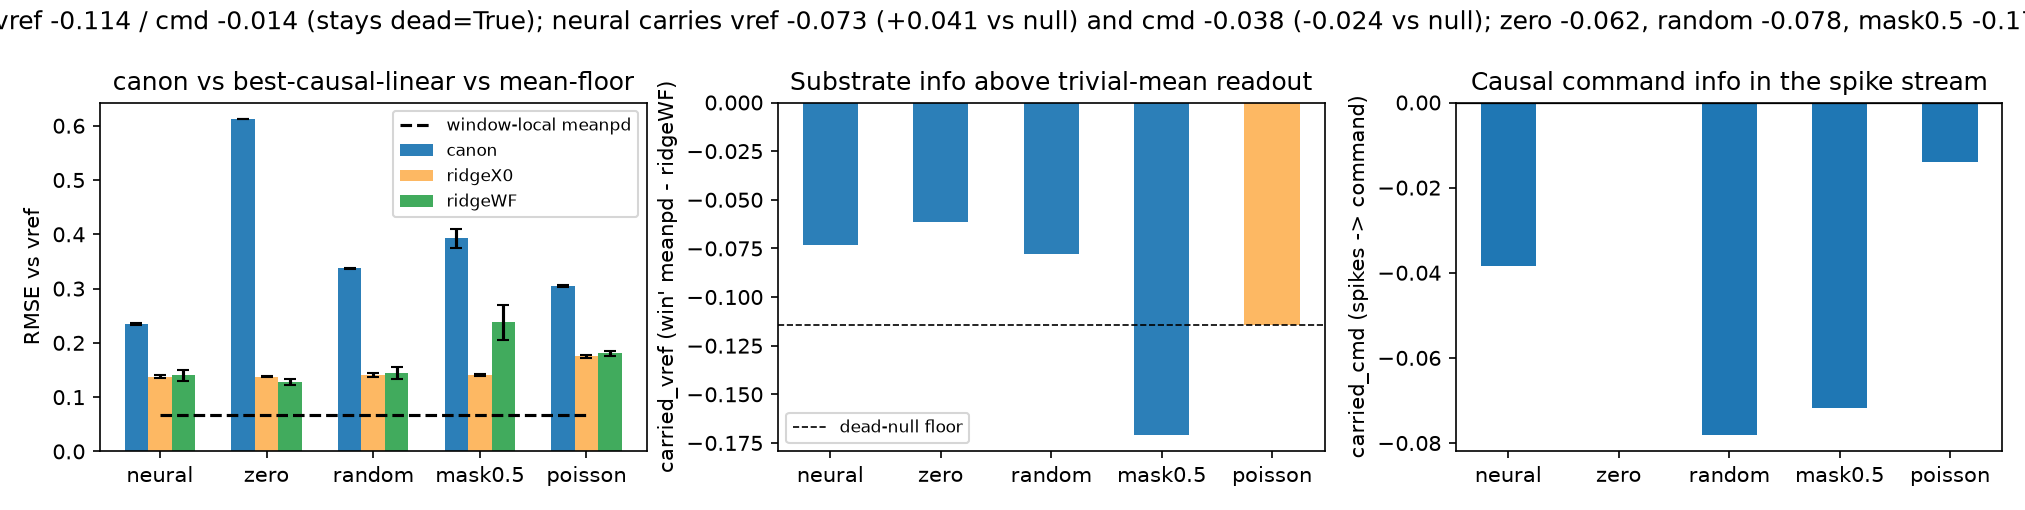
\includegraphics[width=\textwidth]{figures/fig6_gated.png}
\caption{Readout-invariance gate (Gate~D). Left: canonical readout RMSE vs.\
the best causal linear readout and the window-mean floor. Center: carried task
information by mode, with the dead-substrate (poisson) level dashed. Right:
carried spike$\rightarrow$command information. The intact substrate sits
significantly above the dead null on the task and nowhere above it on the
command edge.}
\label{fig:gated}
\end{figure*}

\subsection{Terrain: the loop is not inert}
\label{sec:resD}

Table~\ref{tab:terrain} and Fig.~\ref{fig:terrain} make a deliberately
two-sided point. On the 5\,cm curb, the substrate-mediated loop destabilizes a
step plan the reference policy clears reliably (6/6 down to 1/6 survivors,
Fisher $p=0.0076$ that neural is worse). On rough bumps, the direction
reverses statistically: the reference collapses at the first bump every seed
(0/6), the loop survives 2/6 and always travels farther
(3.89 vs.\ 5.87\,m, Welch $t(5.1)=8.63$, $p=0.0011$). Ramp is survived by all
modes with a measurable speed cost for the closed loop.

This sign-reversal is the strongest single piece of evidence that the loop is
load-bearing rather than cosmetic: an inert decoration could only ride along
with the policy; a genuine substrate-mediated influence changes \emph{which}
walker states are reached, in opposing directions depending on the physical
demand. It also shows the influence is not always beneficial---the honest
statement a fixed decode on a slow substrate deserves.

\begin{table}[t]
\centering
\caption{Terrain battery. Survivors are out of the runs listed; distances in m
(mean$\pm$sd).}
\label{tab:terrain}
\small
\begin{tabular}{llcc}
\toprule
Scene & Mode & Surv. & Distance\\
\midrule
\multirow{2}{*}{ramp ($2^{\circ}$)}
 & reference & 2/2 & 6.23$\pm$0.17\\
 & neural & 2/2 & 4.88$\pm$0.09\\
\multirow{2}{*}{curb 5\,cm}
 & reference & \textbf{6/6} & 6.31$\pm$0.00\\
 & neural & \textbf{1/6} & 5.35$\pm$0.56\\
\multirow{2}{*}{rough bumps}
 & reference & 0/6 & 3.89$\pm$0.06\\
 & neural & \textbf{2/6} & 5.87$\pm$0.56\\
\bottomrule
\end{tabular}
\vspace{2pt}
\begin{flushleft}
\footnotesize
Curb: Fisher $p=0.0076$ (neural $\leq$ reference). Rough distance: Welch
$t(5.1)=8.63$, $p=0.0011$ (neural $>$ reference).
\end{flushleft}
\end{table}

\begin{figure*}[t]
\centering
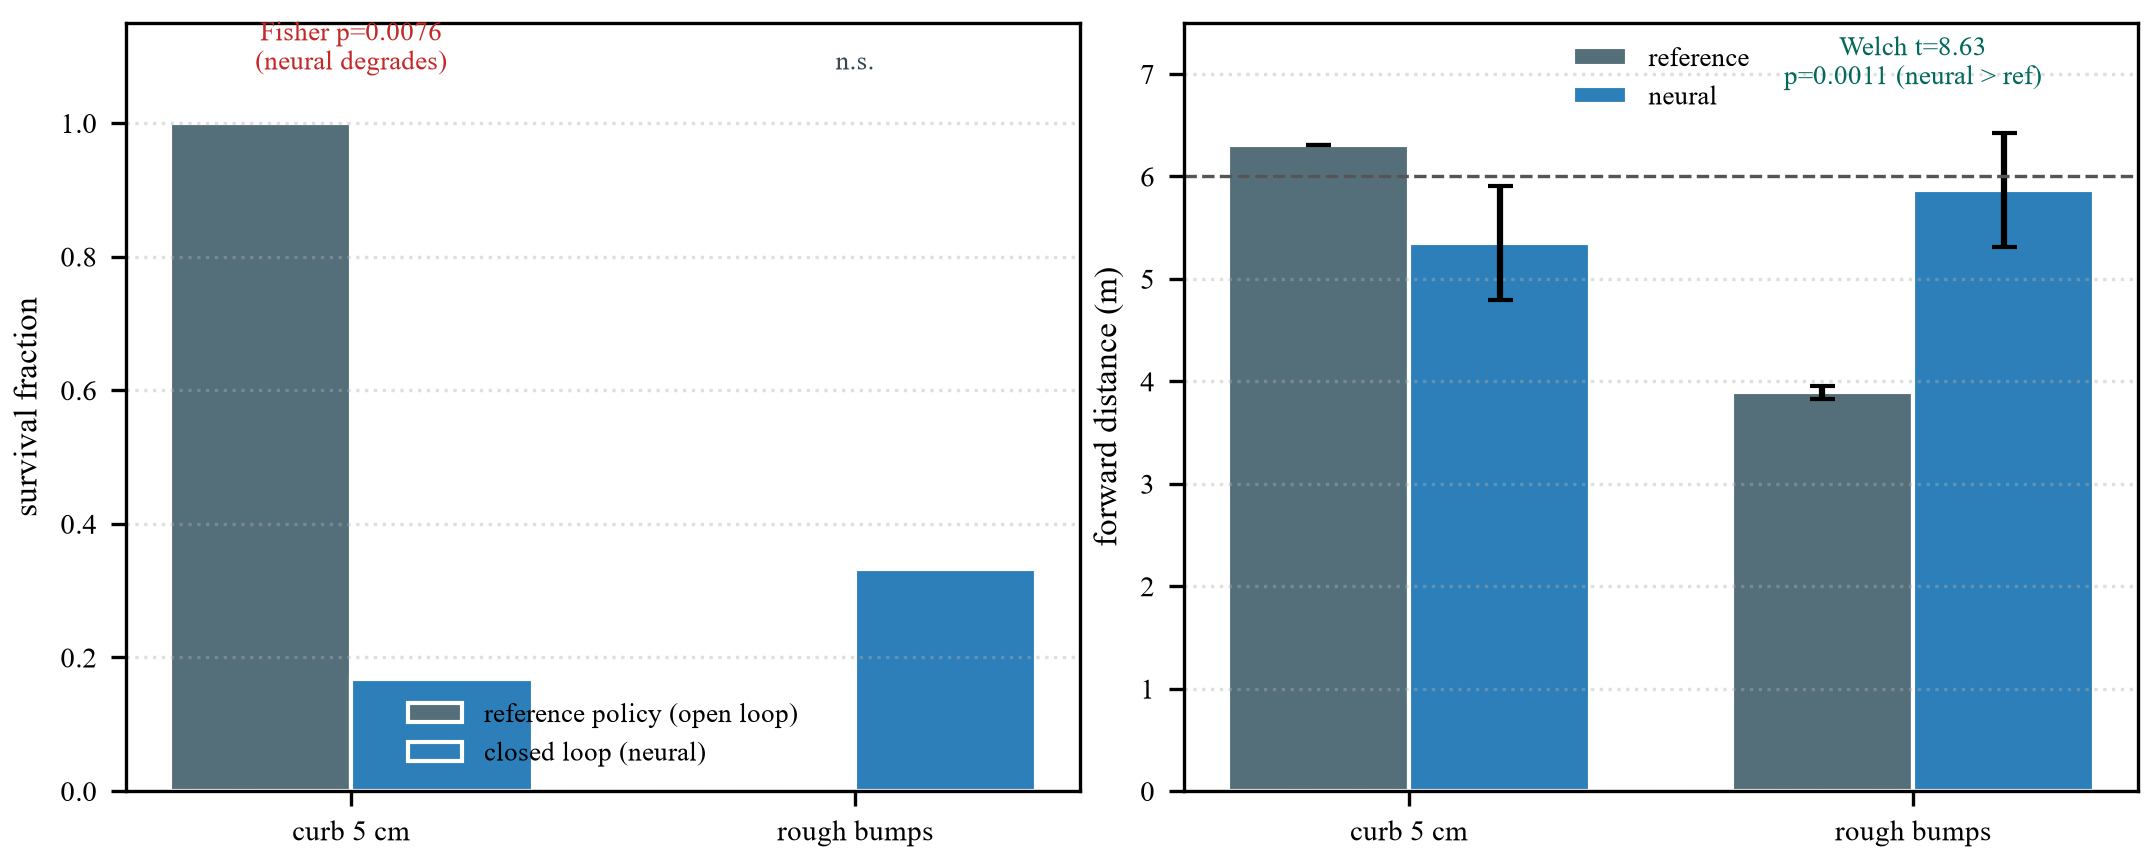
\includegraphics[width=\textwidth]{figures/fig4_terrain.png}
\caption{Terrain batteries. Left: survival fraction; right: traveled distance,
both for reference policy (open loop) and the neural closed loop on the 5\,cm
curb and rough bumps. The loop costs steadiness on the curb and buys balance on
rough ground.}
\label{fig:terrain}
\end{figure*}

\subsection{Authority boundary and information latency}
\label{sec:resE}

\textit{Authority.} The loop's torque channel delivers about
$30\,\mathrm{N\,m}$ of hip-roll correction (0.75 units $\times$
$40\,\mathrm{N\,m/unit}$) against a measured tipping moment of about
$112\,\mathrm{N\,m}$ for a sustained 140\,N lateral push: sustained floor loads
are outside the loop's authority, and every mode---including the torque hub---falls
under them. The lateral impulse frontier is closable for durations
$<0.45\,$s at $\leq140\,$N (the base policy absorbs the impulse; the loop
closes the latency before the instability develops). Longitudinal, a forward
push at 0.3\,s/150\,N falls, while the mirror backward push is survived by all
modes. These numbers bound, rather than flatter, the claim.

\textit{Latency.} The contract tick is 25\,ms and the cadence histograms confirm
the round trip (produce frames $\rightarrow$ read newest $\rightarrow$ decode
$\rightarrow$ stimulate) fits inside it. The information the command is derived
from, however, is up to $1.2\,$s old: the hub integrates a trailing 600-step
window at 2\,ms. The loop is therefore \emph{liquidity}-limited by its
information window, not by its contract tick---the mechanism behind the ramp
speed cost and the curb destabilization, and the reason the rough-ground gain
survives information that is a full gait period old.

\subsection{Information-theoretic summary}

Fig.~\ref{fig:info} summarizes the information-theoretic gate for both
substrates. The causal signature (TE) is nonzero only for the intact loop; it is
exactly zero for the lesioned and dead-substrate modes, and remains at noise for
the uncoupled random decoder.

\begin{figure*}[t]
\centering
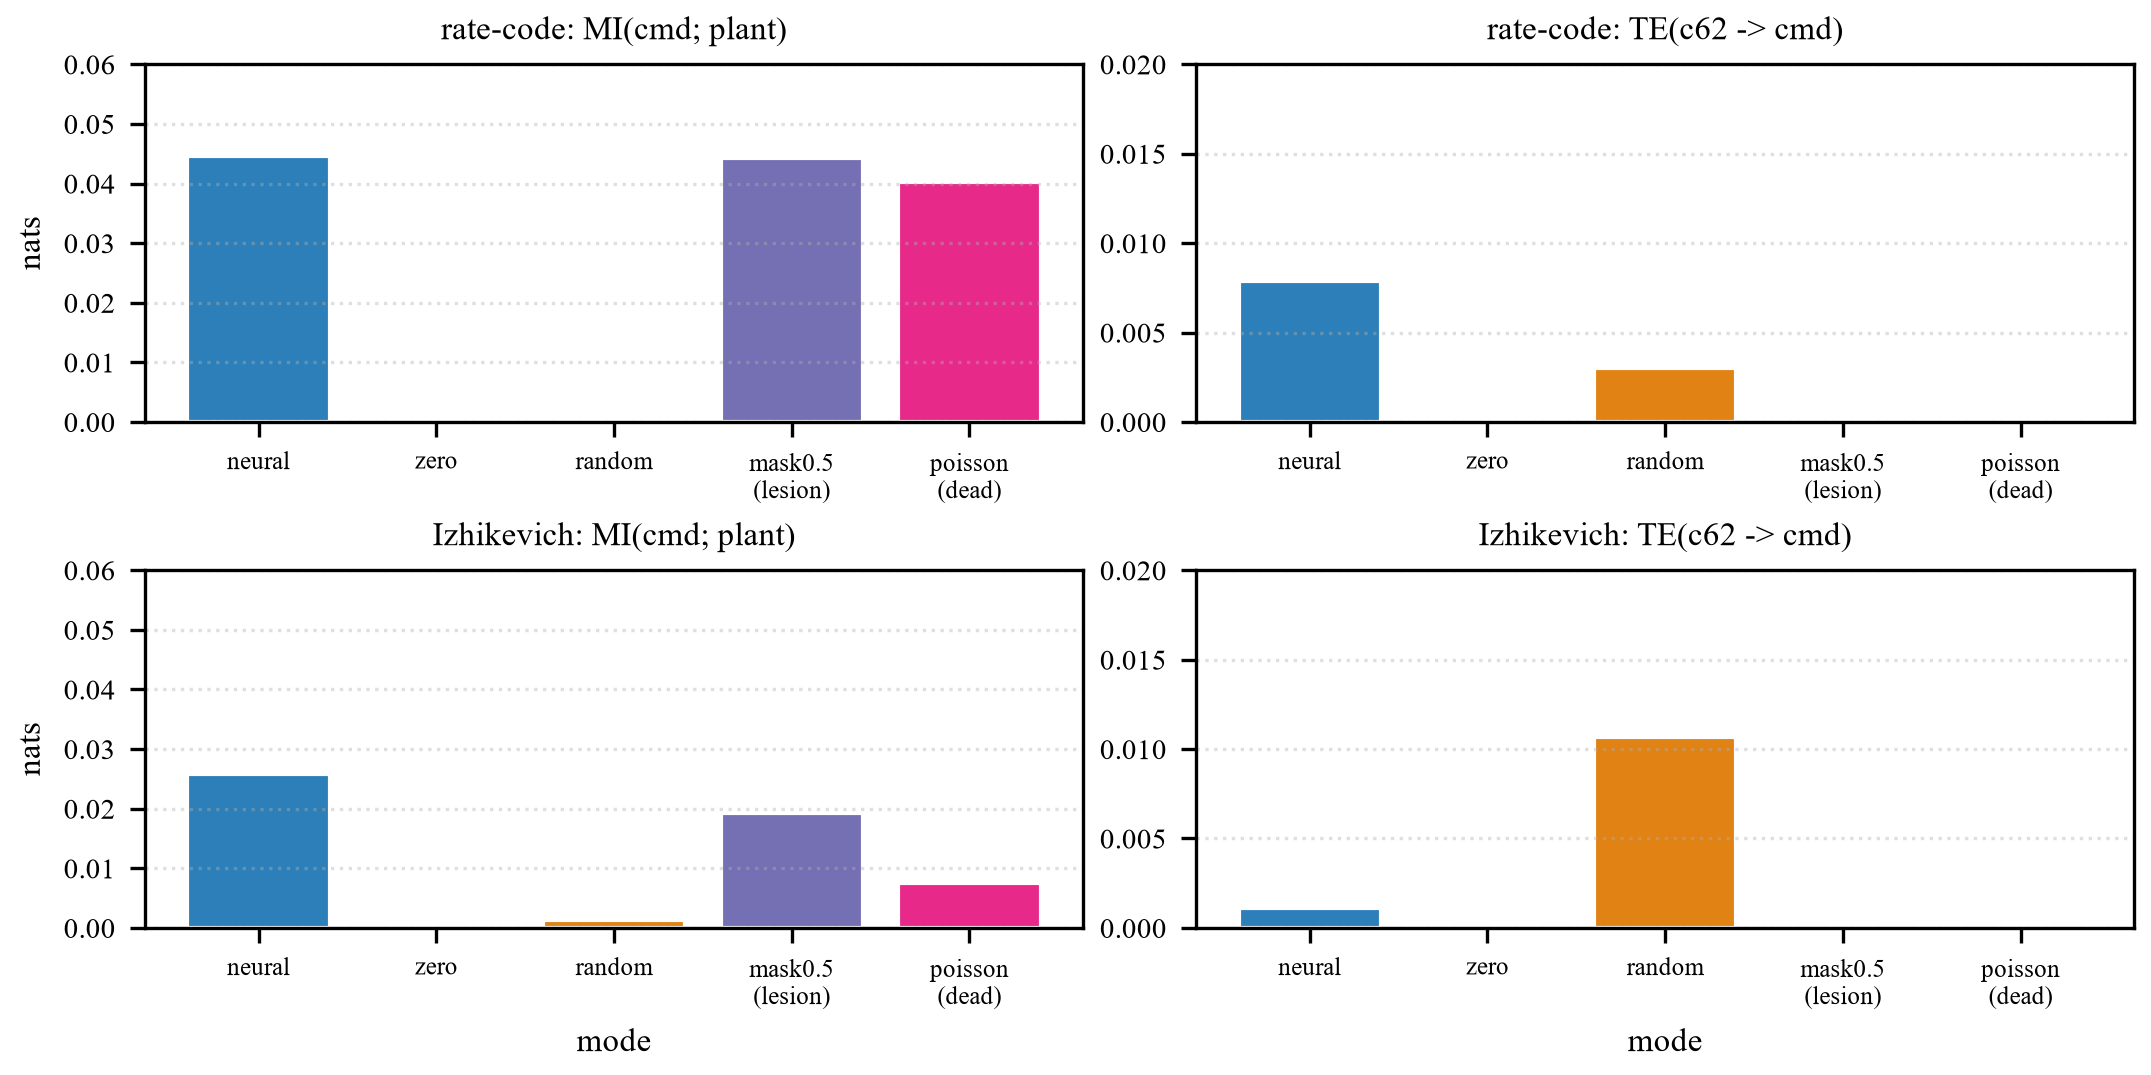
\includegraphics[width=\textwidth]{figures/fig5_information.png}
\caption{Mutual information (left) and transfer entropy (right) for both
substrates. TE along the task channel is the causal signature and is nonzero
only for the intact loop.}
\label{fig:info}
\end{figure*}

\section{Discussion}

The ablation ordering is the argument. \texttt{random} beats \texttt{zero}, so
an \emph{any\ stress} on the command toward the task already buys physical
stability; \texttt{neural} consistently beats the dead substrate, so it is the
information carried by spikes---not their mere presence---that buys the rest;
lesioning 50\,\% of electrodes (which in some seeds erases the task channel)
reverts the loop toward the floor; and switching the pattern generator for a
fully dynamical Izhikevich microcircuit changes nothing in the ordering. Each
branch takes one link out of the loop
(Fig.~\ref{fig:pipeline}) and something measurable breaks.

Two honesty constraints should be stated sharply.

First, the readout is fixed, hand-specified, and nonlinear, and the status of
the information it consumes is measured, not assumed. The closed-loop
readout-invariance gate (Section~\ref{sec:resG}) finds that the best causal
linear readout \emph{cannot} beat a trivial window-mean predictor for any mode,
so the substrate is not readout-invariant; but the intact substrate \emph{does}
carry task information significantly above the statistically matched dead
substrate in both substrates. Load-bearing versus readout-invariant is thus a
measured distinction: ablation destroys the loop's function---that is the
load-bearing claim---while the decodability of the spikes into a command is
explicitly not demonstrated, with the same gate's numbers reported. The
companion open-loop protocol \cite{embodied_neurocomp} that motivated the gate
showed the same distinction open-loop, where apparent tracking of dynamical
microcircuits could collapse under a re-learned readout; here it is a measured
boundary of the closed loop instead of a deferred caveat.

Second, real-time jitter. Because the loop closes in wall clock time, the same
seed can land differently across sessions (hub chunking latency); statistics
therefore use one invocation per (scene, mode, seed), with seeds fixed, and the
$p$-value floor is reported as such rather than padded.

The larger scientific point is methodological. A substrate's value for control
should not be argued from its composition or from a novelty mechanism, but from
whether a load-bearing task is lost when the substrate's information is removed,
and from whether the loop's physical influence is measurable and signed. This
reproducible apparatus provides that test in simulation, at the full contract
of a closed-loop culture platform, with the boundaries stated.

\section{Reproducibility}

All software, configuration, assets (including the vendored robot model and
policy checkpoint), raw per-tick trials, analysis code, and the manuscript are
released together as a single public repository, whose access details are
withheld during the double-anonymous review; pinned dependencies and a
bootstrap script reproduce everything. No biological tissue, and no physical closed-loop platform, is required:
the ``culture substrate'' is simulated in-process, so the entire pipeline runs
from a vendored environment on a CPU-only machine. The repository documents the
exact commands to reproduce the five-by-five battery, the information-theoretic
analyses, the terrain batteries, and the authority envelope, and which committed
JSON files each figure is drawn from. The readout-invariance gate reruns at
full six-seed power from the committed captures via \texttt{src/gate\_d.py}.

\section*{Acknowledgment}

\ifDoubleBlind
\textit{(omitted in the double-anonymous version.)}
\else
The author acknowledges the open-loop falsification protocol
\cite{embodied_neurocomp}, developed in parallel by the author's own research
lane, which shaped the decoder-invariance agenda that the discussion
explicitly leaves to future work.
\fi

\begin{thebibliography}{20}

\bibitem{embodied_neurocomp}
``Embodied Neurocomputation: A Framework for Interfacing Biological Neural
Cultures with Scaled Task-Driven Validation,'' preprint, arXiv:2605.13315,
2026.

\bibitem{kagan2022dishbrain}
B.~J.~Kagan \emph{et al.}, ``In vitro neurons learn and exhibit sentience when
embodied in a simulated game-world,'' \emph{Neuron}, vol.~110, no.~22,
pp.~3952--3969, 2022.

\bibitem{balci2023neurons}
F.~Balc{\i}, S.~Ben~Hamed, T.~Boraud, S.~Bouret, T.~Brochier, C.~Brun,
\emph{et al.}, ``A response to claims of emergent intelligence and sentience in
a dish,'' \emph{Neuron}, vol.~111, no.~5, pp.~604--605, 2023.

\bibitem{kagan2023semantics}
B.~J.~Kagan \emph{et al.}, ``Scientific communication and the semantics of
sentience,'' \emph{Neuron}, vol.~111, no.~5, 2023. [letter]

\bibitem{cai2023brainoware}
H.~Cai \emph{et al.}, ``Brain organoid reservoir computing for artificial
intelligence,'' \emph{Nature Electronics}, vol.~6, pp.~1032--1039, 2023.

\bibitem{maass1997}
W.~Maass, ``Networks of spiking neurons: the third generation of neural network
models,'' \emph{Neural Networks}, vol.~10, no.~9, pp.~1659--1671, 1997.

\bibitem{izhikevich2003}
E.~M.~Izhikevich, ``Simple model of spiking neurons,'' \emph{IEEE Trans.\
Neural Networks}, vol.~14, no.~6, pp.~1569--1572, 2003.

\bibitem{izhikevich2004}
E.~M.~Izhikevich, ``Which model to use for cortical spiking neurons?''
\emph{IEEE Trans.\ Neural Networks}, vol.~15, no.~5, pp.~1063--1070, 2004.

\bibitem{maass2002liquid}
W.~Maass, T.~Natschlaeger, and H.~Markram, ``Real-time computing without stable
states: a new framework for neural computation based on perturbations,''
\emph{Neural Computation}, vol.~14, no.~11, pp.~2531--2560, 2002.

\bibitem{eliasmith2003}
C.~Eliasmith and C.~H.~Anderson, \emph{Neural Engineering: Computation,
Representation, and Dynamics in Neurobiological Systems}. MIT Press, 2003.

\bibitem{bekolay2014}
T.~Bekolay \emph{et al.}, ``Nengo: a Python tool for building large-scale
functional brain models,'' \emph{Frontiers in Neuroinformatics}, vol.~7,
art.~48, 2014.

\bibitem{schreiber2000}
T.~Schreiber, ``Measuring information transfer,'' \emph{Phys.\ Rev.\ Lett.},
vol.~85, no.~2, pp.~461--464, 2000.

\bibitem{kraskov2004}
A.~Kraskov, H.~St{\"o}gbauer, and P.~Grassberger, ``Estimating mutual
information,'' \emph{Phys.\ Rev.\ E}, vol.~69, 066138, 2004.

\bibitem{panzeri2007}
S.~Panzeri, R.~Senatore, M.~A.~Montemurro, and R.~S.~Petersen, ``Correcting for
the sampling bias in spike-train information measures,''
\emph{J.\ Neurophysiology}, vol.~98, pp.~1064--1072, 2007.

\bibitem{walker2018}
B.~L.~Walker and K.~A.~Newhall, ``Inferring information flow in spike-train
data sets using a trial-shuffle method,'' \emph{PLoS ONE}, vol.~13, no.~11,
e0206977, 2018.

\bibitem{theiler1992}
J.~Theiler, S.~Eubank, A.~Longtin, B.~Galdrikian, and J.~D.~Farmer, ``Testing
for nonlinearity in time series: the method of surrogate data,'' \emph{Physica
D}, vol.~58, pp.~77--94, 1992.

\bibitem{ernst2004}
M.~D.~Ernst, ``Permutation methods: a basis for exact inference,''
\emph{Statistical Science}, vol.~19, no.~4, pp.~676--685, 2004.

\bibitem{hurlbert1984}
S.~H.~Hurlbert, ``Pseudoreplication and the design of ecological field
experiments,'' \emph{Ecological Monographs}, vol.~54, no.~2, pp.~187--211,
1984.

\bibitem{georgopoulos1986}
A.~P.~Georgopoulos, A.~B.~Schwartz, and R.~E.~Kettner, ``Neuronal population
coding of movement direction,'' \emph{Science}, vol.~233, pp.~1416--1419, 1986.

\bibitem{quiroga2009}
R.~Q.~Quiroga and S.~Panzeri, ``Extracting information from neuronal
populations: information theory and decoding approaches,'' \emph{Nature Reviews
Neuroscience}, vol.~10, pp.~173--185, 2009.

\bibitem{paninski2004}
L.~Paninski \emph{et al.}, ``Superlinear population encoding of dynamic hand
trajectory in primary motor cortex,'' \emph{J.\ Neuroscience}, vol.~24,
no.~39, pp.~8551--8561, 2004.

\bibitem{todorov2012}
E.~Todorov, T.~Erez, and Y.~Tassa, ``MuJoCo: a physics engine for model-based
control,'' in \emph{Proc.\ IEEE/RSJ Int.\ Conf.\ Intelligent Robots and Systems
(IROS)}, 2012, pp.~5026--5033.

\bibitem{unitree_rl_gym}
Unitree Robotics, \emph{unitree\_rl\_gym: deployment code and pre-trained
policies}, 2024. [Online]. Available:
\url{https://github.com/unitreerobotics/unitree_rl_gym}

\end{thebibliography}

\end{document}